\documentclass{beamer}
\usepackage[utf8]{inputenc}
\usepackage[T1]{fontenc}
\usepackage{graphicx}
\usepackage{color, colortbl}
\usetheme{Frankfurt}
\title[Redmine]{Présentation de Redmine}
\institute{Plateforme de Bioinformatique de Nantes}
\date{5 Février 2012}
\logo{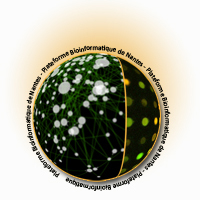
\includegraphics[height=10mm]{image/logo.jpg}}

\usepackage{pslatex}


\setbeamertemplate{caption}[numbered]

\setbeamertemplate{navigation symbols}{
	%    \insertslidenavigationsymbol
	%		\insertframenavigationsymbol
%		\insertsubsectionnavigationsymbol
		\insertsectionnavigationsymbol
	%	\insertdocnavigationsymbol
	%	\insertbackfindforwardnavigationsymbol
}
%foot line page courante/pages totales		
\addtobeamertemplate{footline}{\hfill\insertframenumber/\inserttotalframenumber\hspace{2em}\null}
\beamertemplatetransparentcovered
% Definition des couleures
%\definecolor{LightBlue}{RGB}{0.88,1,1}
\definecolor{LightRed}{RGB}{255,204,204}
\definecolor{LightGreen}{RGB}{153,255,153}

%Sommaire automatique
\AtBeginSection[]{
		\begin{frame}{Sommaire}
		\small \tableofcontents[currentsection, hideothersubsections]
		\end{frame}
	}
\begin{document}

\begin{frame}
	\titlepage
\end{frame}


\section*{Sommaire}
\begin{frame}{Sommaire}
		\small \tableofcontents[hideothersubsections]
\end{frame}

\section[Présentation]{Présentation }
\begin{frame}{Présentation de l'outil}
	\begin{block}{Présentation}
		\begin{itemize}
			\item Redmine est une application Web
			\item Open source (gratuit modifiable)
			\item Flexible : il existe de nombreux plugins
			\item Ajout de fonctionnalités envisageable
		\end{itemize}
	\end{block}

\end{frame}
\begin{frame}{A quoi ça sert ?}
	\begin{block}{Redmine sert à }
		\begin{itemize}
			\item Planifier les projets : Gantt, calendrier, alerte email. 
			\item Travailler de façon collaboratif : Wiki, groupes.
			\item Diffuser du contenu : documents\ldots 
			\item gérer des rapports : synthèse\ldots
		\end{itemize}
	\end{block}
	\begin{alertblock}{Redmine ne sert pas à}
		\begin{itemize}
			 \item à stocker des fichiers (données scientifique)
			 \item à analyser 
			 \item Un LIMS
		\end{itemize}
	\end{alertblock}
\end{frame}

\section[Principe]{Principes}
\subsection{Concepts}
\begin{frame}{Les Concepts}
\begin{block}{Vocabulaire}
	\begin{description}
		\item [Projets - sous projet] : sens large 
		\item [Utilisateurs] : défini par un login mot de passe
		\item [Membres] : utilisateurs contribuant au projet
		\item [Rôles] :  d'un membre pour un projet
		\item [Demandes] : action à faire sur un projet
		\item [Trackers] : type de l'action  à faire
		\item [Status] : progression de la demande, pourcentage réalisé (lié au tracker) 
		\item [Workflow] : enchainement des statuts d'un tracker pour un rôle donné.
	\end{description}

\end{block}
\end{frame}
	\subsection{Projets}
		\begin{frame}{Projets}
			\begin{block}{Création de projet}
				\begin{itemize}
					\item Sens de projet est très large
					\item Définition des membres du projets et de leur rôles.
					\item Ce que voit ou peut faire un utilisateur dépend de son rôle.
					\item Définition du type d'action  (trackers)
				\end{itemize}
			\end{block}
			\begin{block}{Vie d'un projet}
				\begin{itemize}
					\item Faire de nouvelles demandes
					\item Alimenter un wiki
					\item Ajouter du contenu
				\end{itemize}
			\end{block}
		\end{frame}

	

\subsection{Demandes}
\begin{frame}{Les demandes, trackers et workflows}
	\begin{block}{Demande}
		\begin{itemize}		
			\item Une demande est liée à un projet.
			\item Un responsable doit être attribué (peut évoluer au cours de la demande).
			\item Un tracker est associé à la demande.
			\item Le statut de la demande dépend du tracker.
		\end{itemize}
	\end{block}
	\begin{block}{Tracker workflow}
		\begin{itemize}
			\item Un tracker est un type d'action.
			\item Un worklow défini l'enchainement des statuts pour un rôle et un tracker donné.
		\end{itemize}
	\end{block}
\end{frame}
%\section[Interface]{Interface}
%
%\begin{frame}[Interface]{Accueil}
%\begin{figure}
%	\includegraphics[scale=0.15]{redmine1Accueil.png}
%\end{figure}
%\end{frame}
%
%\begin{frame}[Interface]{Ma page}
%\begin{figure}
%	\includegraphics[scale=0.15]{redmine2MaPage.png}
%\end{figure}
%\end{frame}
%
%\begin{frame}[Interface]{Projets}
%	\begin{itemize}
%		\item Ensemble des projets accessibles.	
%	\end{itemize}
%\begin{figure}
%	\includegraphics[scale=0.15]{redmine3Projets.png}
%\end{figure}
%\end{frame}
%
%\begin{frame}[Interface]{Projet : MiccroArray}
%\begin{figure}
%	\includegraphics[scale=0.15]{redmineProjet.png}
%\end{figure}
%\end{frame}
%
%\begin{frame}[Interface]{Sous Projet}
%\begin{figure}
%	\includegraphics[scale=0.15]{Redminesousprojet1.png}
%\end{figure}
%\end{frame}
%
%\begin{frame}[Interface]{Membres du sous projet}
%\begin{figure}
%	\includegraphics[scale=0.15]{redminesousprojet2.png}
%\end{figure}
%\end{frame}
%
%\begin{frame}[Interface]{Sous Projet 3}
%\begin{figure}
%	\includegraphics[scale=0.15]{redminesousprojet3.png}
%\end{figure}
%\end{frame}
%
%\begin{frame}[Interface]{Sous projet 4}
%\begin{figure}
%	\includegraphics[scale=0.15]{redminesousprojet4.png}
%\end{figure}
%\end{frame}
%
%\begin{frame}[Interface]{Sous projet Gant}
%\begin{figure}
%	\includegraphics[scale=0.15]{redminesousprojetGant.png}
%\end{figure}
%\end{frame}
%
%
%\end{frame}

\end{document}

